% !TeX root = surprises.tex

\chapter{Teoremas de geometría y trigonometría}\label{a.trig}

%%%%%%%%%%%%%%%%%%%%%%%%%%%%%%%%%%%%%%%%%%%%%%%%%%%%%%%%%%%%%%%

Este apéndice presenta teoremas de geometría y trigonometría que pueden no ser familiares para el lector, así como teoremas que pueden ser familiares pero cuyas pruebas no lo son.La sección~\ref{a.triangles} presenta tres fórmulas para calcular el área de un triangle. La sección~\ref{a.trig-identities} demuestra las identidades trigonométricas. Aunque las fórmulas y las identidades son en su mayoría familiares, los estudiantes a menudo aprenden estas identidades de memoria o las buscan sin ver nunca una demostración. Las siguientes secciones contienen demostraciones de teoremas avanzados de geometría: Secc.~\ref{a.bisector}---los teoremas de la bisectriz de angles, Secc.~\ref{a.ptolemy}---el teorema de Tolomeo que relaciona los lados y las diagonales de un cuadrilátero circunscrito por una circunferencia, Secc.~ref{a.ceva}---Teorema de Ceva que relaciona los tres segmentos de línea de un triangle, y Sección~\ref{a.menelaus}---Teorema de Menelao sobre los segmentos de una transversal en un triangle.

%%%%%%%%%%%%%%%%%%%%%%%%%%%%%%%%%%%%%%%%%%%%%%%%%%%%%%%%%%%

\section{Teoremas sobre triangles}\label{a.triangles}

%%%%%%%%%%%%%%%%%%%%%%%%%%%%%%%%%%%%%%%%%%%%%%%%%%%%%%%%%%%

\subsection{Cálculo del área de un triangle}
\index{Triangle!computing the area|(}

La fórmula estándar para calcular el área de un triangle a partir de la base y la altura es bien conocida. Se puede demostrar utilizando varios métodos geométricos.

\begin{theorem} El área del triangle $\triangle ABC$ viene dada por:
\begin{align}
\triangle ABC=\frac{1}{2}bh\,,\label{eq.area-from-base}
\end{align}
donde $b$, la base, es uno de los lados del triangle, y $h$, la altura, es la longitud de la altitud a $b$ desde el vértice opuesto (Fig.~\ref{f.area-base-height-1}).
\end{theorem}

\begin{proof}
Figura~\ref{f.area-base-height-2} muestra que ``cortando'' el triangle por la mitad de la altura, podemos ``mover'' los triangles sombreados para formar un rectangle de la misma área que el triangle. La base del rectangle es $b$ y su altura $h/2$.
\end{proof}

\begin{figure}[t]
\begin{minipage}{.45\textwidth}
\begin{center}
\begin{tikzpicture}[scale=.7]
\coordinate (A) at (0,0);
\coordinate (C) at (7,0);
\path[name path=ab] (A) -- +(60:5.5);
\path[name path=cb] (C) -- +(140:7);
\path[name intersections={of=ab and cb,by={B}}];
\draw (A) -- node[below] {$b$} (C) -- node[above] {$a$} (B) -- node[above,xshift=-2pt] {$c$}  cycle;
\node[left] at (A) {$A$};
\node[above right,xshift=4pt] at (A) {$\theta$};
\node[above] at (B) {$B$};
\node[right] at (C) {$C$};
\draw (B) -- node[right,yshift=-4pt] {$h=c\sin\theta$} 
  (B|-A) coordinate (H);
\draw[rotate=90] (H) rectangle +(8pt,8pt);
\end{tikzpicture}
\caption{Cálculo del área de un triangle a partir de la base y la altura}\label{f.area-base-height-1}
\end{center}
\end{minipage}
\hfill
\begin{minipage}{.45\textwidth}
\begin{center}
\begin{tikzpicture}[scale=.7]
\coordinate (A) at (0,0);
\coordinate (C) at (7,0);
\path[name path=ab] (A) -- +(60:5.5);
\path[name path=cb] (C) -- +(140:7);
\path[name intersections={of=ab and cb,by={B}}];
\node[left] at (A) {$A$};
\node[above] at (B) {$B$};
\node[right] at (C) {$C$};
\path (B) -- node[right,near end] {$h/2$} (B|-A) coordinate (H);
\draw[rotate=90] (H) rectangle +(8pt,8pt);
\coordinate (K) at ($(H)!.5!(B)$);
\draw (A) -- node[below] {$b$} (C);
\draw (H) -- (K);
\coordinate (KA) at (K -| A);
\coordinate (KAB) at ($(A)!.5!(B)$);
\fill[color=white!50!red] (A) -- (KA) -- (KAB) -- cycle;
\fill[color=white!50!red] (B) -- (KAB) -- (K) -- cycle;
\coordinate (KC) at (K -| C);
\coordinate (KBC) at ($(B)!.5!(C)$);
\fill[color=white!50!blue] (C) -- (KC) -- (KBC) -- cycle;
\fill[color=white!50!blue] (B) -- (KBC) -- (K) -- cycle;
\draw[very thick,dashed] (A) -- (K -| A) -- (K -| C) -- (C);
\draw[very thick,dashed] (A) -- (B) -- (K);
\draw[very thick,dashed] (B) -- (C);
\path (K) -- node[inner sep=1pt, fill=white,right,
                 xshift=2pt,yshift=-3pt] {$h/2$} (B);
\end{tikzpicture}
\caption{Computation of the area of a triangle from the base and the height}\label{f.area-base-height-2}
\end{center}
\end{minipage}
\end{figure}

\begin{theorem} El área del triangle $\triangle ABC$ viene dada por:
\begin{align}\label{eq.area-from-sine}
\triangle ABC = \frac{1}{2}bc\sin \theta\,.
\end{align}
\end{theorem}
\begin{proof} De Thm.~\ref{eq.area-from-base} usando
$h=c\sin \theta$.
\end{proof}

%%%%%%%%%%%%%%%%%%%%%%%%%%%%%%%%%%%%%%%%%%%%%%%%%%%%%%%%%%%


\index{Triangle!Heron's formula}
\begin{theorem}[Heron] El área del triangle $\triangle ABC$ viene dada por:\label{thm.heron} 
\[
\triangle ABC = \sqrt{s(s-a)(s-b)(s-c)}\,,
\]
donde $s$, el \emph{semi-perímetro} del triangle, es igual a  $\frac{1}{2}(a+b+c)$.
\end{theorem}

\begin{proof}
El radio de una circunferencia y una tangente que corta al radio son perpendiculares. Además, las longitudes de los segmentos de línea de dos tangentes desde el mismo punto al círculo son iguales. Por lo tanto (Fig.~\ref{f.inscribed}):\footnote{Esto demuestra que el \emph{incentro} el centro de la circunferencia inscrita, es la intersección común de las tres bisectrices de los angles.}
\[
\triangle AOB'\cong \triangle AOC',\quad
\triangle BOA'\cong\triangle BOC',\quad
\triangle COA'\cong \triangle COB'\,.
\]
\begin{figure}[ht]
\begin{center}
\begin{tikzpicture}[scale=1.8]
% Draw base and path two lines at known angles
\draw (0,0) coordinate (a) node[xshift=-6pt] {$A$} -- (0:6) coordinate (b) node[xshift=6pt] {$B$};
\path[name path=ac] (a) -- +(50:4);
\path[name path=bc] (b) -- +(150:5);
% Get their intersection and draw lines between vertices
\path[name intersections={of=ac and bc,by=c}];
\node[above] at (c) {$C$};
\draw (a) -- (c) -- (b) -- (a);
% Label angles with tick marks
\draw (a) ++(0:4mm) arc (0:50:4mm);
\draw (a) ++(10:3.5mm) -- +(10:1mm);
\draw (a) ++(15:3.5mm) -- +(15:1mm);
\draw (a) ++(35:3.5mm) -- +(35:1mm);
\draw (a) ++(40:3.5mm) -- +(45:1mm);
\draw (b) ++(150:5mm) arc (150:180:5mm);
\draw (b) ++(157.5:4.5mm) -- +(157.5:1mm);
\draw (b) ++(172.5:4.5mm) -- +(172.5:1mm);
\draw (c) ++(230:3mm) arc (230:330:3mm);
\draw (c) ++(250:2.4mm) -- +(250:.9mm);
\draw (c) ++(255:2.4mm) -- +(255:.9mm);
\draw (c) ++(260:2.4mm) -- +(260:.9mm);
\draw (c) ++(300:2.4mm) -- +(300:.9mm);
\draw (c) ++(305:2.4mm) -- +(305:.9mm);
\draw (c) ++(310:2.4mm) -- +(310:.9mm);
% Path bisectors of two lines
\path[name path=bia] (a) -- +(25:3.5);
\path[name path=bib] (b) -- +(165:5);
% Intersection of angle bisectors
\path [name intersections={of=bia and bib,by=center}];
% Draw angle bisectors to center
\draw (a) -- (center);
\draw (c) -- (center);
\draw (b) -- (center);
% Draw radii
\draw (center) -- node[left] {$r$} ($(a)!(center)!(b)$) node[below,yshift=-2pt] {$C'$} coordinate (ap);
\draw (center) -- node[left,yshift=-4pt] {$r$} ($(a)!(center)!(c)$) node[above left] {$B'$} coordinate (bp);
\draw (center) -- node[right] {$r$} ($(b)!(center)!(c)$) node[above right] {$A'$} coordinate (cp);
% Draw dots
\vertex{center};
\node[above,xshift=3pt,yshift=7pt] at (center) {$O$};
% Draw right angle squares
\draw (ap) -- ++(90:4pt) -- ++(0:4pt) -- ++(-90:4pt);
\draw (bp) -- ++(-40:4pt) -- ++(-130:4pt) -- ++(-220:4pt);
\draw (cp) -- ++(-30:4pt) -- ++(-120:4pt) -- ++(-210:4pt);
% Labels of angles
\node[above,xshift=5pt,yshift=18pt] at (center) {$\gamma/2$};
\node[above left,xshift=-4pt,yshift=18pt] at (center) {$\gamma/2$};
\node[above right,xshift=3pt,yshift=-3pt] at (center) {$\beta/2$};
\node[below right,yshift=-3pt] at (center) {$\beta/2$};
\node[left,xshift=-5pt,yshift=2pt] at (center) {$\alpha/2$};
\node[below left,xshift=2pt,yshift=-4pt] at (center) {$\alpha/2$};
% Labels of line segments (names of points are weird...)
\path (a) -- node[below,yshift=-2pt] {$u$} (ap);
\path (a) -- node[left, xshift=-2pt] {$u$} (bp);
\path (b) -- node[above,yshift=2pt]  {$v$} (cp);
\path (b) -- node[below,xshift=-2pt] {$v$} (ap);
\path (c) -- node[above,xshift=-2pt] {$w$} (bp);
\path (c) -- node[above,xshift=2pt]  {$w$} (cp);
% Labels of sides
\draw[<->] ($(a)+(0,-10pt)$) -- node[fill=white] {$c$} 
           ($(b)+(0,-10pt)$);
\draw[<->] ($(a)+(-10pt,8pt)$) -- node[fill=white] {$b$}
           ($(c)+(-10pt,8pt)$);
\draw[<->] ($(b)+(6pt,10pt)$) -- node[fill=white] {$c$}
           ($(c)+(6pt,10pt)$);
% Inscribed circle
\node[very thick,dotted,draw,circle through=(ap)] at (center) {};
\end{tikzpicture}
\end{center}
\caption{Triangle con un círculo inscrito}\label{f.inscribed}
\end{figure}
El área $\triangle ABC$ es la suma de los seis triangles anteriores. Como la altura de los seis triangles es $r$, el radio de la circunferencia inscrita, obtenemos:
\begin{subeqnarray}
\triangle ABC&=&\triangle AOB'\!+\!\triangle AOC'\!+\!\triangle BOA'\!+\!\triangle BOC'\!+\!\triangle COA'\!+\!\triangle COB'\\
\triangle ABC&=&\frac{1}{2}r(u+u+v+v+w+w)\\
\triangle ABC&=&\frac{1}{2}r(a+b+c)\\
\triangle ABC&=&rs \slabel{eq.area-heron}\,.
\end{subeqnarray}

Definamos ahora los lados en función de las tangentes de los angles centrales:
\begin{displaymath}
\tan \frac{\alpha}{2} = \frac{u}{r},\quad
\tan \frac{\beta}{2} = \frac{v}{r},\quad
\tan \frac{\gamma}{2} = \frac{w}{r}\,.
\end{displaymath}
A partir de estas definiciones y $s=\frac{1}{2}(2u+2u+2w)$ obtenemos:
\[
s = u+v+w = r\left(\tan \frac{\alpha}{2}+\tan \frac{\beta}{2}+\tan \frac{\gamma}{2}\right)\,.
\]
Desde $\frac{\alpha}{2}+\frac{\alpha}{2}+\frac{\beta}{2}+\frac{\beta}{2}+\frac{\gamma}{2}+\frac{\gamma}{2}=360^\circ$ y así $\frac{\alpha}{2}+\frac{\beta}{2}+\frac{\gamma}{2}=180^\circ$, por Thm.~\ref{thm.tangent3}:
\begin{eqnarray*}
s&=&r\left(\tan \frac{\alpha}{2}\tan \frac{\beta}{2}\tan \frac{\gamma}{2}\right)\\
&=&r\left(\frac{u}{r}\frac{v}{r}\frac{w}{r}\right)=\frac{1}{r^2}(u\,v\,w)\\
r&=&\sqrt{\displaystyle\frac{u\,v\,w}{s}}\,.
\end{eqnarray*}
Por Eq.~\ref{eq.area-heron}:
\[
\triangle ABC=rs=s\sqrt{\displaystyle\frac{u\,v\,w}{s}}=\sqrt{s\,u\,v\,w}\,.
\]
La fórmula de Heron se deduce de $u=s-a, v=s-b, w=s-c$.
\end{proof}
\index{Triangle!computing the area|)}

%%%%%%%%%%%%%%%%%%%%%%%%%%%%%%%%%%%%%%%%%%%

\section{Identidades trigonométricas}\label{a.trig-identities}
\index{Trigonometric identities|(}
\index{Trigonometric identities!sine and cosine of the sum and difference of two angles}

%%%%%%%%%%%%%%%%%%%%%%%%%%%%%%%%%%%%%%%%%%%%%%%%%%%%%%%%%%%

\subsection{El seno y el coseno de la suma y la diferencia de dos angles} \label{s.sum-of-trig}

\begin{theorem}\label{thm.sum-of-trig}
\begin{eqnarray*}
\sin(\alpha+\beta) &=& \sin\alpha\cos\beta + \cos\alpha\sin\beta\\
\sin(\alpha-\beta) &=& \sin\alpha\cos\beta - \cos\alpha\sin\beta\\
\cos(\alpha+\beta) &=& \cos\alpha\cos\beta - \sin\alpha\sin\beta\\
\cos(\alpha-\beta) &=& \cos\alpha\cos\beta + \sin\alpha\sin\beta\,.
\end{eqnarray*}
\end{theorem}
Demostraremos la primera fórmula; las demás fórmulas pueden obtenerse utilizando los valores del seno y coseno para $-\alpha$ y $90^\circ-\alpha$.

Dado un triangle rectangle $\triangle ABC$ con angle agudo $\alpha$ y un triangle rectangle $\triangle ACD$ con angle agudo $\beta$, podemos unirlos para obtener figuras geométricas con angle $\alpha+\beta$ (Fig.~\ref{f.sin-sum1}). El diagrama de la izquierda es el más utilizado en las demostraciones de las identidades. Aquí damos dos pruebas basadas en los diagramas central y derecho.
\begin{figure}[h]
\begin{center}
\begin{tikzpicture}[scale=.85]
\coordinate (A) at (0,0);
\node[below] at (A) {$A$};
\node[right,xshift=6pt,yshift=4pt] at (A) {$\alpha$};
\node[above right,xshift=6pt,yshift=8pt] at (A) {$\beta$};
\coordinate (B) at (3,0);
\node[below] at (B) {$B$};
\path[name path=ac1] (A) -- +(40:4.5);
\path[name path=bc1] (B) -- +(90:3.5);
\path[name intersections={of=ac1 and bc1,by={C}}];
\node[above right] at (C) {$C$};
\draw (A) -- (B) -- (C) -- cycle;
\draw (C) -- ($(C)!2cm!-90:(A)$) coordinate (D) -- (A);
\node[above] at (D) {$D$};
\draw[rotate=90] (B) rectangle +(7pt,7pt);
\draw[rotate=128] (C) rectangle +(7pt,7pt);

\begin{scope}[xshift=4.3cm]
\coordinate (B) at (0,0);
\node[below] at (B) {$B$};
\coordinate (D) at (4,0);
\node[below] at (D) {$D$};
\draw (B) -- +(70:4) coordinate (A);
\node[above] at (A) {$A$};
\draw (A) -- (B) -- (D) -- cycle;

\draw (A) -- (A|-B) coordinate (C);
\node[below] at (C) {$C$};
\node[below left,xshift=2pt,yshift=-18pt] at (A) {$\alpha$};
\node[below right,xshift=0pt,yshift=-14pt] at (A) {$\beta$};
\draw[rotate=90] (C) rectangle +(7pt,7pt);
\draw (C) rectangle +(7pt,7pt);
\end{scope}

\begin{scope}[xshift=9.75cm]
\coordinate (A) at (0,0);
\node[below] at (A) {$A$};
\node[right,xshift=6pt,yshift=5pt] at (A) {$\alpha$};
\node[above right,xshift=4pt,yshift=8pt] at (A) {$\beta$};
\coordinate (B) at (3.5,0);
\node[below] at (B) {$B$};
\draw (A) -- +(70:4.5) coordinate (D);
\node[above] at (D) {$D$};
\path[name path=dc1] (D) -- +(-20:2.5);
\path[name path=bc1] (B) -- +(90:4);
\path[name intersections={of=dc1 and bc1,by={C}}];
\node[above] at (C) {$C$};
\draw[rotate=90] (B) rectangle +(7pt,7pt);
\draw[rotate=-110] (D) rectangle +(7pt,7pt);
\draw (A) -- (B) -- (C) -- (D) -- cycle;
\draw (A) -- (C);
\end{scope}
\end{tikzpicture}
\end{center}
\caption{Diagramas para demostrar la identidad del seno de sumas de angles}\label{f.sin-sum1}
\end{figure}

\begin{proof}
\mbox{}\\
(1)
Calculemos el área del $\triangle ABD$ de dos formas distintas: (1) utilizando la Ec.~\ref{eq.area-from-sine} sobre el $\triangle ABD$, y (2) utilizando la ecuación por separado sobre el $\triangle ABC$ y el $\triangle ADC$ (Fig.~\ref{f.sin-sum2}).
$h$ también se calcula dos veces utilizando la definición de las funciones trigonométricas:
\begin{eqnarray*}
\triangle ABD &=& \frac{1}{2}bc\sin(\alpha+\beta)\\
\triangle ABD &=& \triangle ABC+\triangle ADC\\
&=& \frac{1}{2}ch\sin \alpha + \frac{1}{2}bh\sin \beta\\
&=& \frac{1}{2}c(b\cos\beta)\sin \alpha + \frac{1}{2}b(c\cos\alpha)\sin \beta\,.
\end{eqnarray*}
Igualando las dos fórmulas para $\triangle ABD$ y cancelando $\frac{1}{2}bc$, obtenemos:
\[
\sin(\alpha+\beta)=\sin\alpha\cos\beta+\cos \alpha\sin\beta\,.
\]
\end{proof}

\begin{figure}[tb]
\begin{center}
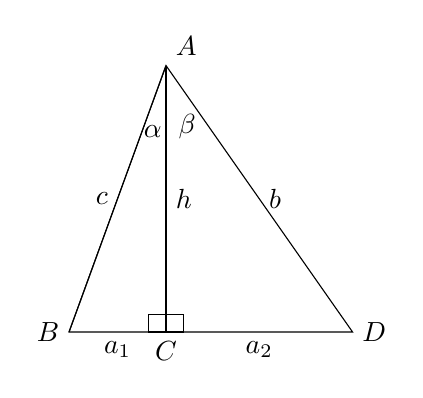
\begin{tikzpicture}[scale=.9]
\coordinate (B) at (0,0);
\node[left] at (B) {$B$};
\coordinate (D) at (4,0);
\node[right] at (D) {$D$};
\draw (B) -- +(70:4) coordinate (A);
\node[above right] at (A) {$A$};
\draw (A) -- node[left] {$c$} (B) -- (D) -- node[right] {$b$} cycle;

\draw (A) -- node[right] {$h$} (A|-B) coordinate (C);
\node[below] at (C) {$C$};
\node[below left,xshift=2pt,yshift=-18pt] at (A) {$\alpha$};
\node[below right,xshift=1pt,yshift=-14pt] at (A) {$\beta$};
\draw[rotate=90] (C) rectangle +(7pt,7pt);
\draw (C) rectangle +(7pt,7pt);
\path (B) -- node[below] {$a_1$} (C) -- node[below] {$a_2$} (D);
\end{tikzpicture}
\end{center}
\caption{Cálculo del área de un triangle de dos maneras}\label{f.sin-sum2}
\end{figure}

La segunda prueba utiliza el siguiente teorema:
\begin{theorem}
En un círculo de \emph{diámetro} $1$ la longitud de una cuerda que subtiende un angle inscrito es igual al seno del angle (Fig.~\ref{f.chord-angle}).
\end{theorem}

\begin{figure}[b]
\begin{center}
\begin{tikzpicture}[scale=.7]

\coordinate (A) at (0,0);
\coordinate (C) at (3,4);
\coordinate (O) at ($(A)!.5!(C)$);
\vertex{O};
\node[left] at (O) {$O$};
\draw (A) -- (C);
\node[draw,circle through=(A),name path=circle] at (O) {};
\coordinate (B) at ($(O)+(10:2.5)$);
\draw (A) -- (B) -- node[left] {$a$} (C);
\draw[rotate=120] (B) rectangle +(8pt,8pt);
\coordinate (D) at ($(O)+(160:2.5)$);
\draw(C) -- (D) -- (B);
\node[above right,xshift=12pt,yshift=12pt] at (A) {$\alpha$};
\node[right,xshift=16pt,yshift=2pt] at (D) {$\alpha$};
\node[below left] at (A) {$A$};
\node[above right] at (C) {$B$};
\node[right] at (B) {$C$};
\node[left] at (D) {$D$};
\end{tikzpicture}
\end{center}
\caption{Todos los angles inscritos subtendidos por una cuerda son iguales}\label{f.chord-angle}
\end{figure}

\begin{proof}
Sea $\overline{AB}$ un diámetro y $\angle BAC=\alpha$. Sea $D$ cualquier otro punto de la circunferencia que forme un triangle $\triangle BDC$, uno de cuyos lados es la cuerda $\overline{BC}$. Como cuerdas iguales subtienden angles inscritos iguales $\angle BDC=\alpha$. En el triangle rectangle $\triangle ABC$:
\[
\sin \alpha = \frac{\overline{BC}}{\overline{AB}}=\frac{\overline{BC}}{1}=\overline{BC}\,.
\]
\end{proof}

\begin{proof}
\mbox{}\\
(2)
Esta prueba se basa en el diagrama de la derecha de la Fig.~\ref{f.sin-sum1} reproducido en la Fig.~\ref{f.trig-quad-circle}, donde el cuadrilátero $\overline{ABCD}$ ha sido inscrito en una circunferencia.
Por Thm.~\ref{thm.quad-circum} un cuadrilátero puede ser circunscrito\index{Círculo circunscrito} por un círculo si y sólo si la suma de cada par de angles opuestos es $180^\circ$.
$\angle ADC+\angle ABC=180^\circ$ ya que ambos angles son rectos. Por Thm.~\ref{thm.interior-angles-of-a-polygon} la suma de los angles interiores de un cuadrilátero es $360^\circ$, por lo que $\angle DAB+\angle DCB=180^\circ$. 
\begin{figure}[t]
\begin{center}
\begin{tikzpicture}[scale=.8]
\coordinate (A) at (0,0);
\node[left] at (A) {$A$};
\node[right,xshift=6pt,yshift=5pt] at (A) {$\alpha$};
\node[above right,xshift=4pt,yshift=8pt] at (A) {$\beta$};
\coordinate (B) at (3.5,0);
\node[right] at (B) {$B$};
\draw (A) -- +(70:4.5) coordinate (D);
\node[above left] at (D) {$D$};
\path[name path=dc1] (D) -- +(-20:2.5);
\path[name path=bc1] (B) -- +(90:4);
\path[name intersections={of=dc1 and bc1,by={C}}];
\node[above right] at (C) {$C$};
\draw[rotate=90] (B) rectangle +(9pt,9pt);
\draw[rotate=-110] (D) rectangle +(9pt,9pt);
\draw (A) -- (B) -- (C) -- (D) -- cycle;
\draw (A) -- (C);
\draw (D) -- (B);

\coordinate (O) at ($(A)!.5!(C)$);
\node[draw,circle through=(A),name path=circle] at (O) {};
\node[below right,xshift=6pt,yshift=-4pt] at (D) {$\alpha$};
\node[below,xshift=1pt,yshift=-10pt] at (D) {$\gamma$};
\node[below left,xshift=-6pt,yshift=4pt] at (C) {$\delta$};
\node[below,xshift=-4pt,yshift=-6pt] at (C) {$\gamma$};
\node[above left,xshift=-7pt,yshift=4pt] at (B) {$\delta$};
\node[above,xshift=-4pt,yshift=14pt] at (B) {$\beta$};
\end{tikzpicture}
\end{center}
\caption{Un cuadrilátero circunscrito por un círculo}\label{f.trig-quad-circle}
\end{figure}

Sea el diámetro de la circunferencia $1$ (si no, multiplica todo por la longitud del diámetro). Entonces los lados del cuadrilátero son:
\[
\overline{BC}=\sin\alpha,\quad \overline{CD}=\sin\beta,\quad \overline{AB}=\sin\gamma,\quad \overline{DA}=\sin\delta\,,
\]
y sus diagonales son:
\[
\overline{BD}=\sin(\alpha + \beta),\quad \overline{CA}=\sin (\alpha+\gamma)\,.
\]

Por el Teorema de Ptolomeo (Thm.~\ref{thm.ptolemy}) el producto de las diagonales de un cuadrilátero circunscrito por una circunferencia es igual a la suma de los productos de los lados opuestos del cuadrilátero. Como $\angle ADC$ y $\angle ABC$ son angles rectos tenemos:
\[
\renewcommand{\arraystretch}{1.3}
\begin{array}{lcl}
\sin (\alpha+\beta)\sin(\alpha+\gamma)&=&
\sin \alpha \sin\delta + \sin \beta\sin \gamma\\
\sin (\alpha+\beta)\sin(90^\circ)&=&
\sin \alpha \sin(90^\circ-\beta) + \sin \beta\sin (90^\circ-\alpha)\\
\sin (\alpha+\beta)&=&\sin\alpha\cos\beta+\cos\alpha\sin \beta\,.
\end{array}
\]
\end{proof}

%%%%%%%%%%%%%%%%%%%%%%%%%%%%%%%%%%%%%%%%%%%%%%%%%%%%%%%%%%%

\subsection{Coseno de un angle triple}\label{s.cosine}
\index{Trigonometric identities!cosine of a triple angle}
\begin{theorem}\label{thm.triple-angle}
\[
\cos 3\alpha=4\cos^3\alpha -3\cos\alpha\,.
\]
\end{theorem}
\begin{proof}
La prueba utiliza las fórmulas en Thm.~\ref{thm.sum-of-trig} y la fórmula $\sin^2\alpha+\cos^2\alpha=1$:
\begin{eqnarray*}
\cos 3\alpha &=& \cos (2\alpha +\alpha)\\
&=& \cos 2\alpha\cos\alpha - \sin 2\alpha\sin\alpha\\
&=& (\cos^2\alpha -\sin^2\alpha)\cos\alpha - (2\sin\alpha\cos\alpha)\sin\alpha\\
&=&\cos^3\alpha - \cos\alpha\sin^2\alpha -2\sin^2\alpha\cos\alpha)\\
&=&\cos^3\alpha - \cos\alpha +\cos^3\alpha -2\cos\alpha+2\cos^3\alpha\\
&=&4\cos^3\alpha -3\cos\alpha\,.
\end{eqnarray*}
\end{proof}

%%%%%%%%%%%%%%%%%%%%%%%%%%%%%%%%%%%%%%%%%%%%%%%%%%%%%%%%%%%

\subsection{El seno y el coseno de un semiangle}\label{s.sine-cosine-half}
\index{Trigonometric identities!sine and cosine of a half-angle}
\begin{theorem}\label{thm.sine-cosine-half}
Si $\alpha$ es un angle en un \emph{triangle} entonces:\footnote{La fórmula general es más compleja porque las raíces cuadradas pueden ser positivas o negativas dependiendo del cuadrante en el que se encuentre $\alpha/2$. Para un triangle $0\!<\!\alpha\!<\!180^\circ$, entonces $0\!<\!\alpha/2\!<\!90^\circ$ está en el primer cuadrante y tanto el seno como el coseno son positivos.}
\begin{eqnarray*}
\cos \left(\frac{\alpha}{2}\right)&=&\sqrt{\frac{1+\cos\alpha}{2}}\\
\sin\left(\frac{\alpha}{2}\right)&=&\sqrt{\frac{1-\cos\alpha}{2}}\,.
\end{eqnarray*}
\end{theorem}

\begin{proof}
La prueba utiliza las fórmulas Thm.~\ref{thm.sum-of-trig} y la fórmula $\sin^2\alpha+\cos^2\alpha=1$:
\begin{eqnarray*}
\cos \alpha&=&\cos 2\left(\frac{\alpha}{2}\right)=\cos \left(\frac{\alpha}{2}\right)\cos\left(\frac{\alpha}{2}\right)-\sin \left(\frac{\alpha}{2}\right)\sin\left(\frac{\alpha}{2}\right)\\
&=&2\cos^2 \left(\frac{\alpha}{2}\right)-1\\
\cos \left(\frac{\alpha}{2}\right)&=&\sqrt{\frac{1+\cos\alpha}{2}}\\
\sin^2\left(\frac{\alpha}{2}\right)&=& 1-\cos^2\left(\frac{\alpha}{2}\right)=1-\frac{1+\cos\alpha}{2}\\
\sin \left(\frac{\alpha}{2}\right)&=&\sqrt{\frac{1-\cos\alpha}{2}}\,.
\end{eqnarray*}
\end{proof}

%%%%%%%%%%%%%%%%%%%%%%%%%%%%%%%%%%%%%%%%%%%%%%%%%%%%%%%%%%%

\subsection{La ley de los cosenos}

\begin{theorem}[Law of cosines]
En un triangle $\triangle ABC$ de lados $a,b,c$ (Fig.~\ref{f.law-cosines2}):\label{thm.law-of-cosines}\index{Law of cosines}
\[
c^2=a^2+b^2-2ab\cos \angle ACB\,.
\]
\end{theorem}

\begin{proof}
\mbox{}\\
(1)
Dejar caer una altura desde $C$ hasta $\overline{AB}$ y utilizar la definición de coseno y el Teorema de Pitágoras:
\begin{subeqnarray}
c&=& x+(c-x)=a\cos \beta + b\cos \alpha\\
c^2&=&ac\cos \beta + bc\cos \alpha\,.\slabel{eq.lc1}
\end{subeqnarray}
Del mismo modo, baje las altitudes de $A$ a $\overline{BC}$ y de $B$ a $\overline{AC}$ para obtener:
\begin{subeqnarray}
a^2&=&ca\cos \beta + ba\cos \gamma\slabel{eq.lc2}\\
b^2&=&cb\cos \alpha + ab\cos \gamma\,.\slabel{eq.lc3}
\end{subeqnarray}

Sumando las Ecs.~\ref{eq.lc2} y \ref{eq.lc3} y restando la Ec.~\ref{eq.lc1} se obtiene:
\begin{eqnarray*}
a^2+b^2-c^2&=&ca\cos \beta + ba\cos \gamma\\
&&\;\; +\,cb\cos \alpha + ab\cos \gamma \\
&&\;\; -\,ac\cos \beta - bc\cos \alpha\\
&=&2ab\cos \gamma\\
c^2&=&a^2+b^2-2ab\cos \gamma\,.
\end{eqnarray*}
\end{proof}

\begin{figure}[b]
\begin{center}
\begin{tikzpicture}[scale=.65]
  \coordinate[label = left:$A$] (A) at (0,0);
  \coordinate[label = right:$B$] (B) at (6,0);
  \draw (A) -- (40:5) coordinate (C) node[above] {$C$};
  \draw (A) -- (B) -- node[right] {$a$} (C) -- node[left,yshift=4pt,xshift=-2pt] {$b$} cycle;
\node[below,xshift=-4pt,yshift=-6pt] at (C) {$\gamma$};
\node[above right,xshift=8pt] at (A) {$\alpha$};
\node[above left,xshift=-8pt] at (B) {$\beta$};
\coordinate (D) at (A-|C);
\draw (C) -- (D);  
\draw (D) rectangle +(10pt,10pt);
\draw[<->] (0,-.5) -- node[fill=white] {$c$} (6,-0.5);
\draw[<->] (0,-1) -- node[fill=white] {$c-x$} ($(D)+(0,-1)$);
\draw[<->] ($(D)+(0,-1)$) -- node[fill=white] {$x$} (6,-1);
\end{tikzpicture}
\caption{Prueba 1 de la ley de los cosenos}\label{f.law-cosines2}
\end{center}
\end{figure}

\begin{proof}
\mbox{}\\
(2)
La segunda prueba utiliza el teorema de Ptolomeo (Thm.~\ref{thm.ptolemy}).\footnote{¡La sección~\ref{a.ptolemy} utiliza la Ley de los Cosenos para demostrar el teorema de Ptolomeo! La primera prueba de la Ley de los Cosenos evita este razonamiento circular. Además, hay pruebas del teorema de Ptolomeo que no utilizan la Ley de los Cosenos.}

El triangle $\triangle ABC$ puede circunscribirse en una circunferencia. 
Construir otro triangle $\triangle ABC'$ congruente con $\triangle ABC$ e inscrito en la misma circunferencia (Fig.~\ref{f.law-cosines3}). Esto se puede hacer mediante la construcción de un angle de $\overline{AB}$ igual a $\angle CAB$ que se cruza con el círculo en $C'$ y luego construir la línea $\overline{C'A}$.
Como los angles subtendidos por la misma cuerda son iguales $\angle AC'B =\angle BCA$, entonces también $\angle CBA=\angle C'AB$ y así $\triangle ABC'\cong\triangle BAC$ por angle-lado-angle con el lado común $\overline{AB}$.

Caen perpendiculares de $C$ a $D$ y de $C'$ a $D'$ sobre $\overline{AB}$ de modo que $x=a\cos \beta$. Por el teorema de Ptolomeo para el cuadrilátero $\overline{ABCC'}$:
\begin{eqnarray*}
b^2&=&a^2+c(c-2x)\\
&=& a^2 + c(c-2a\cos\beta)\\
&=&a^2+c^2-2ac\cos\beta\,.
\end{eqnarray*}
\end{proof}

\begin{figure}[b]
\begin{center}
\begin{tikzpicture}[scale=.8]
\coordinate (origin) at (0,0);
\coordinate (A) at (-3,-1.5);
\coordinate (B) at (3,-1.5);
\node[draw,circle through=(A),name path=circle] at (origin) {};
\node[left] at (A) {$A$};
\node[right] at (B) {$B$};
\path[name path=b1] (A) -- +(40:7cm);
\path[name path=b2] (B) -- +(140:7cm);
\path [name intersections={of=circle and b1,by={C}}];
\node[above] at (C) {$C$};
\path [name intersections={of=circle and b2,by={Cp}}];
\node[above] at (Cp) {$C'$};
\draw (A) -- node[below] {$c$} (B) -- node[right] {$a$} (C) -- node[left,yshift=4pt,xshift=-2pt] {$b$} cycle;
\draw (A) -- (B) -- node[right,yshift=4pt,xshift=2pt] {$b$}(Cp) -- node[left] {$a$} cycle;
\draw (C) -- node[above] {$c-2x$} (Cp);
\coordinate (D) at (C|-B);
\coordinate (Dp) at (Cp|-B);
\draw (C) -- (D);
\draw[rotate=90] (D) rectangle +(8pt,8pt);
\draw (Cp) -- (Dp);
\draw (Dp) rectangle +(8pt,8pt);
\draw[<->] ($(A)+(0,-.8)$) -- node[fill=white] {$x$} ($(Dp)+(0,-.8)$);
\draw[<->] ($(Dp)+(0,-.8)$) -- node[fill=white] {$c-2x$} ($(D)+(0,-.8)$);
\draw[<->] ($(D)+(0,-.8)$) -- node[fill=white] {$x$} ($(B)+(0,-.8)$);
\node[below] at (D) {$D$};
\node[below] at (Dp) {$D'$};
\node[above right,xshift=8pt,yshift=6pt] at (B) {$\beta$};
\draw ($(B)+(-.8,0)$) arc (180:104:.8);
\draw[->] ($(B)+(.4,.5)$) -- +(190:1.12);

\node[above left,xshift=-8pt,yshift=6pt] at (A) {$\beta$};
\draw ($(A)+(.8,0)$) arc (0:76:.8);
\draw[->] ($(A)+(-.4,.5)$) -- +(-10:1.12);
\end{tikzpicture}
\end{center}
\caption{Prueba 2 de la ley de los cosenos}\label{f.law-cosines3}
\end{figure}                       

%%%%%%%%%%%%%%%%%%%%%%%%%%%%%%%%%%%%%%%%%%%%%%%%%%%%%%%%%%%

\subsection{La tangente de la suma de dos ángulos}\label{s.tangent-sum}
\index{Trigonometric identities!tangent of the sum of two angles}

\begin{theorem}\label{thm.tangent-sum}
\[
\tan (\alpha+\beta) =\frac{\tan\alpha+\tan\beta}{1-\tan\alpha\tan\beta}\,.
\]
\end{theorem}

\begin{proof}

\begin{eqnarray*}
\tan (\alpha+\beta) &=& \frac{\sin(\alpha+\beta)}{\cos(\alpha+\beta)}\\
&=&\frac{\sin\alpha\cos\beta+\cos\alpha\sin\beta}{\cos\alpha\cos\beta-\sin\alpha\sin\beta}\\
&=&\frac{\sin\alpha+\cos\alpha\tan\beta}{\cos\alpha-\sin\alpha\tan\beta}\\
&=&\frac{\tan\alpha+\tan\beta}{1-\tan\alpha\tan\beta}\,.
\end{eqnarray*}

\end{proof}

%%%%%%%%%%%%%%%%%%%%%%%%%%%%%%%%%%%%%%%%%%%%%%%%%%%%%%%%%%%

\subsection{La tangente de un semiángulo}\label{s.tangent-half}
\index{Trigonometric identities!tangent of a half-angle}
\begin{theorem}\label{thm.tangent-half}
\[
\tan\left(\frac{\alpha}{2}\right) = \frac{-1\pm\sqrt{1+\tan^2\alpha}}{\tan\alpha}\,.
\]
\end{theorem}
\begin{proof}
Deducimos y resolvemos una ecuación cuadrática en $\displaystyle\tan\left(\displaystyle\frac{\alpha}{2}\right)$:
\begin{displaymath}
\begin{array}{lll}
\tan \alpha&=&\displaystyle\frac{
  \tan\left(\displaystyle\frac{\alpha}{2}\right)+
  \tan\left(\displaystyle\frac{\alpha}{2}\right)
  }{
  1-\tan\left(\displaystyle\frac{\alpha}{2}\right)
    \tan\left(\displaystyle\frac{\alpha}{2}\right)
  }\\
\tan\alpha \tan^2  \left(\displaystyle\frac{\alpha}{2}\right) + 2 \tan \left(\displaystyle\frac{\alpha}{2}\right) -\tan\alpha &=&0\\
\tan\left(\displaystyle\frac{\alpha}{2}\right) &=& \displaystyle\frac{-1\pm\sqrt{1+\tan^2\alpha}}{\tan\alpha}\,.
\end{array}
\end{displaymath}
\end{proof}

%%%%%%%%%%%%%%%%%%%%%%%%%%%%%%%%%%%%%%%%%%%%%%%%%%%%%%%%%%%

\subsection{El producto de tres tangentes}\label{s.tangent-three}
\index{Trigonometric identities!product of three tangents}
\begin{theorem}\label{thm.tangent3}
If $\alpha+\beta+\gamma=180^\circ$ then:
\[
\tan\alpha+\tan\beta+\tan\gamma = \tan\alpha\tan\beta\tan\gamma\,.
\]
\end{theorem}

\begin{proof}
\begin{eqnarray*}
\tan\gamma &=& \tan (180^\circ-(\alpha+\beta))\\
&=& -\tan (\alpha+\beta)\\
&=& -\frac{\tan\alpha+\tan\beta}{1-\tan\alpha\tan\beta}\\
\tan\alpha\tan\beta\tan\gamma &=&\tan\alpha+\tan\beta+\tan\gamma\,.
\end{eqnarray*}
\end{proof}

%%%%%%%%%%%%%%%%%%%%%%%%%%%%%%%%%%%%%%%%%%%%%%%%%%%%%%%%%%%

\begin{figure}[b]
\begin{center}
\begin{tikzpicture}[scale=.7]
\coordinate (o1) at (0,0);
\coordinate (a1) at (1.8,0);
\node[draw, name path = circle] at (o1)
    [circle through = (a1)] {};
\foreach \node/\angle in {a2/120,a3/240} {
  \coordinate (\node) at (\angle:1.8);
}
\draw (a1) -- (a2) -- (a3) -- cycle;
\begin{scope}[xshift=5cm]
\coordinate (o2) at (0,0);
\coordinate (b1) at (1.8,0);
\node[draw, name path = circle] at (o2)
    [circle through = (b1)] {};
\foreach \node/\angle in
  {b2/45,b3/90,b4/135,b5/180,b6/-135,b7/-90,b8/-45} {
  \coordinate (\node) at (\angle:1.8);
}
\draw (b1) -- (b2) -- (b3) -- (b4) -- (b5) -- (b6) -- (b7) -- (b8) -- cycle;
\end{scope}
\begin{scope}[xshift=10cm]
\coordinate (o3) at (0,0);
\coordinate (c1) at (1.8,0);
\node[draw, name path = circle] at (o3)
    [circle through = (c1)] {};
\foreach \node/\angle in
  {c2/22.5,c3/45,c4/67.5,c5/90,c6/112.5,c7/135,
   c8/157.5,c9/180,c16/-22.5,c15/-45,c14/-67.5,
   c13/-90,c12/-112.5,c11/-135,c10/-157.5} {
  \coordinate (\node) at (\angle:1.8);
}
\draw (c1) -- (c2) -- (c3) -- (c4) -- (c5) -- (c6) --
  (c7) -- (c8) -- (c9) -- (c10) -- (c11) -- (c12) -- (c13) --
  (c14) -- (c15) -- (c16) -- cycle;
\end{scope}
\end{tikzpicture}
\caption{Polígonos regulares con lados de $3$, $8$ y $16$ inscritos en un círculo}\label{fig.regular-polygons}
\end{center}
\end{figure}

\subsection{El límite de $\sin\alpha/\alpha$}\label{s.sin-over-x}
\index{Trigonometric identities!limit@limit of $\sin \alpha/\alpha$}

\begin{theorem}\label{thm.limit-sine-over}
\[
\lim_{\alpha\rightarrow 0}\frac{\sin\alpha}{\alpha}=1\,.
\]
\end{theorem}

\begin{proof}
Al examinar los polígonos regulares inscritos en un círculo (Fig.~\ref{fig.regular-polygons}), vemos que cuantos más lados tiene un polígono, más se acerca su perímetro a la circunferencia del círculo. La circunferencia del círculo dividida por el número de lados es la longitud de un arco con los mismos puntos extremos que el lado correspondiente, ya que en un polígono regular todos los lados tienen la misma longitud. Dado que la relación entre la circunferencia del círculo y el perímetro de un polígono inscrito se aproxima a $1$ a medida que aumenta el número de lados, también lo hace la relación entre la longitud de un arco y la cuerda correspondiente. Esto se demuestra con los siguientes ejemplos numéricos:
\[
\begin{array}{r@{\hspace{10pt}}r@{\hspace{10pt}}r@{\hspace{10pt}}r}
\hline
\textrm{Angle} & \textrm{Arc length} & \textrm{Chord length} & \textrm{Ratio}\\\hline
80 & 1.396 & 1.286  & 1.090\\
60 & 1.047 & 1.000  & 1.047\\
40 & 0.698 & 0.684 & 1.006\\
5  & 0.087 & 0.087 &1.000 \\\hline
\end{array}
\]
Dado que $a=b=1$ la longitud de la cuerda $c$ que subtiende a $\alpha$ puede calcularse a partir de la Ley de los Cosenos \index{Ley de los cosenos} (Fig.~\ref{fig.length-of-a-chord}):
\begin{figure}[t]
\begin{center}
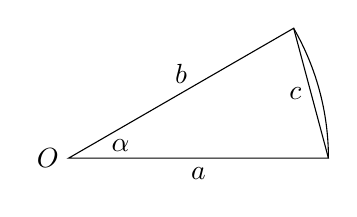
\begin{tikzpicture}[scale=1.1]
  \coordinate  (A) at (3,0);
  \coordinate[label = left:$O$] (O) at (0,0);
  \vertex{O};
  \draw (A) arc(0:30:3) coordinate (B);
  \draw (A) -- node[below] {$a$} (O) -- node[above] {$b$} (B) -- node[left] {$c$} cycle;
  \node[above right,xshift=12pt,yshift=-1pt] at (O) {$\alpha$};
\end{tikzpicture}
\caption{La longitud de una cuerda correspondiente a un arco de tamaño $\alpha$}\label{fig.length-of-a-chord}
\end{center}
\end{figure}
\begin{eqnarray*}
c^2&=&a^2+b^2-2ab\cos \alpha\\
c&=&\sqrt{2-2\cos \alpha}\\
\lim_{\alpha\rightarrow 0} c&=& \sqrt{2-2\cdot 1}=0\,.
\end{eqnarray*}
En referencia a Fig.~\ref{fig.ratio-of-sine-to-x}:
\[
\lim_{\alpha \rightarrow 0} \frac{\sin \alpha}{\alpha} = \lim_{\alpha \rightarrow 0} \frac{2\sin \alpha}{2\alpha}\,.
\]
Es la relación entre la longitud de la cuerda $\overline{PQ}$ y la longitud del arco $\widehat{PQ}$.
Pero hemos visto que esta relación converge a $1$ como el ángulo subtendido $2\alpha$ tiende a $0$, así:
\[
\lim_{\alpha \rightarrow 0} \frac{\sin \alpha}{\alpha} = 1\,.
\]
\end{proof}
\index{Trigonometric identities|)}

\begin{figure}[h]
\begin{center}
\begin{tikzpicture}[scale=.9]
  \draw[thin] (-2,0) -- (2,0);
  \draw[thin] (0,-2) -- (0,2);
  \coordinate[label = above left:$A$]  (A) at (-2,0);
  \coordinate[label = above right:$B$] (B) at (2,0);
  \coordinate[label = above left:$O$] (O) at (0,0);
\vertex{O};
  \node[above right,xshift=6pt] at (O) {$\alpha$} 
    node[below right,xshift=6pt] {$\alpha$};
  \coordinate (P) at (40:2);
  \node[above right] at (P) {$P$};
  \coordinate (Q) at (-40:2);
  \node[draw, name path = circle] at (O)
    [circle through = (A)] {};
  \draw (B)
    arc[start angle=0,end angle=40,radius=2cm];
  \draw (B)
    arc[start angle=0,end angle=-40,radius=2cm];
  \node at (2.1,.8) {$\alpha$};
  \node at (2.1,-.8) {$\alpha$};
  \draw[<->] (P) -- node[fill=white,xshift=-4pt] {$\sin \alpha$}
    (P |- O) coordinate (D);
  \draw[<->] (D) -- node[fill=white,xshift=-4pt] {$\sin \alpha$} (Q);
  \node[below right] at (Q) {$Q$};
  \draw (Q) -- node[below] {$1$} (O) -- node[above] {$1$} (P);
\end{tikzpicture}
\caption{Relación entre $\sin x$ y $x$}\label{fig.ratio-of-sine-to-x}
\end{center}
\end{figure}

%%%%%%%%%%%%%%%%%%%%%%%%%%%%%%%%%%%%%%%%%%%%%%%%%%%%%%%%%%%

\section{Teoremas de la bisectriz del ángulo}\label{a.bisector}
\index{Triangle!angle bisector theorem}

\begin{theorem}\label{thm.angle-bisector}
En $\triangle ABC$ que la bisectriz del ángulo de $\angle BAC$ intersecan $\overline{BC}$ en $D$ (Fig.~\ref{f.angle-bisector}). Entonces:
\[
\frac {\overline{BD}}{\overline{CD}}=\frac {\overline{AB}}{\overline{AC}}\,.
\]
\end{theorem}

\begin{figure}[b]
\begin{center}
\begin{tikzpicture}[scale=.8]
% Draw base and path two lines at known angles
\draw (0,0) coordinate (b) node[left] {$B$} -- (8,0) coordinate (c) node[right] {$C$};
\path[name path=ba] (b) -- +(50:4.5);
\path[name path=ca] (c) -- +(150:7);
% Get their intersection and draw lines between vertices
\path[name intersections={of=ba and ca,by=a}];
\node[above] at (a) {$A$};
\draw (a) -- (c) -- (b) -- (a);
\path[name path=bc] (b) -- (c);
\path[name path=bisector] (a) -- +(-80:4);
\path[name intersections={of= bc and bisector,by=d}];
\node[below] at (d) {$D$};
\draw (a) -- (d);
\node[below left,xshift=2pt,yshift=-8pt] at (a) {$\alpha$};
\node[below right,xshift=2pt,yshift=-8pt] at (a) {$\alpha$};
\draw (a) -- node[left] {$h$} (a |- b);
\draw (a|-b) rectangle +(7pt,7pt);
\end{tikzpicture}
\end{center}
\caption{Teorema de la bisectriz interna del ángulo}\label{f.angle-bisector}
\end{figure}
\begin{proof}
Demostramos el teorema calculando las áreas de dos triángulos utilizando tanto la base y la altura (Ec.~\ref{eq.area-from-base}), como la base, el ángulo y el lado (Ec.~\ref{eq.area-from-sine}):
\begin{eqnarray*}
\triangle ABD&=&\frac{1}{2}\overline{BD}h=\frac{1}{2}\overline{AB}\,\overline{AD}\sin \alpha\\
\frac{\overline{BD}}{\overline{AB}}&=&\frac{\overline{AD}\sin \alpha}{h}\\
\triangle ACD&=&\frac{1}{2}\overline{CD}h=\frac{1}{2}\overline{AC}\,\overline{AD}\sin \alpha\\
\frac{\overline{CD}}{\overline{AC}}&=&\frac{\overline{AD}\sin \alpha}{h}\\
\frac{\overline{BD}}{\overline{CD}}&=&\frac{\overline{AB}}{\overline{AC}}\,.
\end{eqnarray*}
\end{proof}

También existe un teorema de la bisectriz del ángulo para la \emph{bisectriz externa}:
\index{Triangle!angle bisector theorem}
\begin{theorem}\label{thm.external-angle-bisector}
In $\triangle ABC$ sea $\overline{AE}$ la bisectriz del ángulo suplementario al ángulo $\triangle BAC$ (Fig.~\ref{f.angle-bisector-external}) y que la bisectriz intersecte a $\overline{BC}$ en $E$ (Fig.~\ref{f.angle-bisector}). Entonces:
\[
\frac {\overline{BE}}{\overline{CE}}=\frac {\overline{AB}}{\overline{AC}}\,.
\]
\end{theorem}

\begin{figure}[t]
\begin{center}
\begin{tikzpicture}[scale=1]
% Draw base and path two lines at known angles
\draw (0,0) coordinate (b) node[below] {$B$} -- (6,0) coordinate (c) node[right] {$C$};
\path[name path=ba] (b) -- +(70:2.5);
\draw[name path=ca] (c) -- +(160:7);
% Get their intersection and draw lines between vertices
\path[name intersections={of=ba and ca,by=a}];
\node[above] at (a) {$A$};
\draw (a) -- (c) -- (b) -- (a);
\path[name path=bc] (b) -- (c);
\node[left,xshift=-10pt,yshift=-2pt] at (a) {$\alpha$};
\node[below,xshift=-12pt,yshift=-8pt] at (a) {$\alpha$};
\path[name path=ext-bisector] (a) -- +(-155:4.7);
\draw[name path=ext-bc] (c) -- ($(c)!1.6!(b)$);
\path[name intersections={of=ext-bc and ext-bisector,by=e}];
\draw (a) -- (e) node[below] {$E$};
\coordinate (d) at (a |- b);
\draw (a) -- node[right] {$h$} (d);
\draw (d) rectangle +(6pt,6pt);
\end{tikzpicture}
\end{center}
\caption{Teorema de la bisectriz del ángulo exterior}\label{f.angle-bisector-external}
\end{figure}

\begin{proof} Dado que $\overline{AC}$ es una línea recta $\angle EAC=180^\circ-\alpha$.
\begin{eqnarray*}
\triangle ABE&=&\frac{1}{2}\overline{BE}h=\frac{1}{2}\overline{AE}\,\overline{AB}\sin \alpha\\
\triangle ACE&=&\frac{1}{2}\overline{CE}h=\frac{1}{2}\overline{AE}\,\overline{AC}\sin (180^\circ-\alpha)=\frac{1}{2}\overline{AE}\,\overline{AC}\sin \alpha\\
\frac{\overline{BE}}{\overline{AB}}&=&\frac{\overline{AE}\sin \alpha}{h}=\frac{\overline{CE}}{\overline{AC}}\\
\frac{\overline{BE}}{\overline{CE}}&=&\frac{\overline{AB}}{\overline{AC}}\,.
\end{eqnarray*}
\end{proof}

%%%%%%%%%%%%%%%%%%%%%%%%%%%%%%%%%%%%%%%%%%%%%%%%%%%%%%%%%%%

\section{Teorema de Ptolomeo}\label{a.ptolemy}
\index{Ptolemy's theorem}

%%%%%%%%%%%%%%%%%%%%%%%%%%%%%%%%%%%%%%%%%%%%%%%%%%%%%%%%%%%

\subsection{Trapecio circunscrito por una circunferencia}\label{s.circumscribed}

Antes de demostrar el teorema de Ptolomeo, demostraremos teoremas sobre cuadriláteros y trapecios.

\begin{theorem}\label{thm.quad-circum}
Un cuadrilátero puede ser circunscrito por una circunferencia si y sólo si los ángulos opuestos son suplementarios (suma a $180^\circ$).
\end{theorem}\index{Circumscribed circle}

Los libros de texto de geometría ofrecen una prueba sencilla de la dirección de avance, pero es difícil encontrar una prueba de la inversa, por lo que aquí se ofrecen ambas pruebas.

\begin{proof}
\mbox{}\\
(Dirección de avance)
Un ángulo inscrito es igual a la mitad del arco que lo subtiende por lo que $\angle DAB$ es la mitad del arco $\widehat{DCB}$ y $\angle DCB$ es la mitad del arco $\widehat{DAB}$ (Fig.~\ref{f.trap-1}). Los dos arcos forman toda la circunferencia del círculo por lo que su suma es $360^\circ$. Por lo tanto, $\angle DAB + \angle DCB = \frac{1}{2} \cdot 360^\circ = 180^\circ$, y análogamente $\angle ADC + \angle ABC = 180^\circ$.
\end{proof}

\begin{figure}[tb]
\begin{minipage}{.45\textwidth}
\begin{center}
\begin{tikzpicture}[scale=.55]
\coordinate (origin) at (0,0);
\coordinate (A) at (1,3);
\node[draw,circle through=(A),name path=circle] at (origin) {};
\node[above right] at (A) {$A$};
\path[name path=b] (A) -- (-50:4.5cm);
\path[name path=c] (A) -- (-120:4.5cm);
\path[name path=d] (A) -- (150:4.5cm);
\path [name intersections={of=circle and b,by={b1,B}}];
\node[right] at (B) {$B$};
\path [name intersections={of=circle and c,by={c1,C}}];
\node[below left] at (C) {$C$};
\path [name intersections={of=circle and d,by={d1,D}}];
\node[above left] at (D) {$D$};
\draw (A) -- (B) -- (C) -- (D) -- cycle;
\end{tikzpicture}
\caption{Un cuadrilátero circunscrito por un círculo}\label{f.trap-1}
\end{center}
\end{minipage}
\hfill
\begin{minipage}{.45\textwidth}
\begin{center}
\begin{tikzpicture}[scale=.55]
\coordinate (origin) at (0,0);
\coordinate (A) at (1,3);
\node[draw,circle through=(A),name path=circle] at (origin) {};
\node[above right] at (A) {$A$};
\path[name path=b] (A) -- (-50:4cm);
\path[name path=c] (A) -- (-120:4cm);
\path[name path=d] (A) -- (150:4cm);
\path [name intersections={of=circle and b,by={b1,B}}];
\node[right] at (B) {$B$};
\path [name intersections={of=circle and c,by={c1,C}}];
\node[below left] at (C) {$C$};
\path [name intersections={of=circle and d,by={d2,D}}];
\node[above left] at (D) {$D$};
\coordinate (Cp) at ($(C)!.2!(D)$);
\draw (A) -- (B) -- (Cp) -- (D) -- cycle;
\node[left,xshift=1pt,yshift=2pt] at (Cp) {$C'$};
\draw (D) -- (B) -- (C) -- (Cp);
\end{tikzpicture}
\caption{El cuarto vértice debe estar en la circunferencia}\label{f.trap-2}
\end{center}
\end{minipage}
\end{figure}

\begin{proof}
\mbox{}\\
(Dirección inversa)
Cualquier triángulo puede ser circunscrito por una circunferencia. Circunscribimos $\triangle DAB$ por una circunferencia y supongamos que $C'$ es un punto tal que $\angle DAB + \angle DC'B = 180^\circ$, pero $C'$ está \emph{not} en la circunferencia del círculo. Sin pérdida de generalidad, que $C'$ esté dentro de la circunferencia (Fig.~\ref{f.trap-2}).

Construir una semirrecta que prolongue $\overline{DC'}$ y que $C$ sea su intersección con la circunferencia. Entonces $\overline{ABCD}$ está circunscrita por una circunferencia:\index{Circumscribed circle}
\begin{eqnarray*}
\angle DAB + \angle DCB &=&  180^\circ = \angle DAB + \angle DC'B\\
\angle DCB &=& \angle DC'B\,,
\end{eqnarray*}
lo cual es imposible si $C$ está en el círculo y $C'$ está dentro del círculo.
\end{proof}

\begin{theorem}\label{thm.isoceles-trapezoid}
Los ángulos opuestos de un trapecio isósceles son suplementarios.
\end{theorem}
\begin{proof}
Construir la recta $\overline{AB'}$ paralela a $\overline{CD}$ (Fig.~\ref{f.trap-3}). $\overline{AB'CD}$ es un paralelogramo y $\triangle ABB'$ es un triángulo isósceles, por lo que $\angle C= \angle ABB' = \angle AB'B = \angle B$. Análogamente, $\angle A = \angle D$. Como la suma de los ángulos internos de cualquier cuadrilátero es igual a $360^\circ$:
\begin{eqnarray*}
\angle A + \angle B + \angle C + \angle D &=& 360^\circ\\
2\angle A + 2 \angle C &=& 360^\circ\\
\angle A +  \angle C &=& 180^\circ\,,
\end{eqnarray*}
and similarly $\angle B +  \angle D = 180^\circ$.
\end{proof}

\begin{theorem}
Un trapecio isoceles puede ser circunscrito por un círculo.
\end{theorem}
La prueba es inmediata por Thms.~\ref{thm.quad-circum}, \ref{thm.isoceles-trapezoid}.

\begin{figure}[t]
\begin{center}
\begin{tikzpicture}[scale=.65]
\clip (-4.5,-2) rectangle (4.5,2.8);
\coordinate (origin) at (0,0);
\coordinate (A) at (2.5,1.8);
\node[circle through=(A),name path=circle] at (origin) {};
\node[above right] at (A) {$A$};
\path[name path=b] (A) -- ++(-80:4cm);
\path[name path=d] (A) -- ++(180:6cm);
\path [name intersections={of=circle and b,by={b1,B}}];
\node[below right] at (B) {$B$};
\path [name intersections={of=circle and d,by={d1,D}}];
\node[above left] at (D) {$D$};
\path[name path=c] (D) -- ++(-100:4cm);
\path [name intersections={of=circle and c,by={c1,C}}];
\node[below left] at (C) {$C$};
\draw (A) -- node[right] {$x$} (B);
\draw[name path=bc] (B) -- node[below] {$y$} (C);
\draw (C) -- node[left] {$x$} (D) -- node[above] {$y$} (A);
\path[name path=para] (A) -- ++(-100:4cm);
\path [name intersections={of=para and bc,by={Bp}}];
\node[below left] at (Bp) {$B'$};
\draw (A) -- node[left,xshift=-2pt] {$x$} (Bp);
\end{tikzpicture}
\end{center}
\caption{Un trapecio isoceles}\label{f.trap-3}
\end{figure}

%%%%%%%%%%%%%%%%%%%%%%%%%%%%%%%%%%%%%%%%%%%%%%%%%%%%%%%%%%%

\subsection{Demostración del teorema de Ptolomeo}

\begin{theorem}[Ptolomeo]Dado un cuadrilátero circunscrito por una circunferencia, la siguiente fórmula relaciona las longitudes de las diagonales y las longitudes de los lados (Fig.~\ref{f.trig-ptolemy}).\label{thm.ptolemy}\index{Circumscribed circle}
\[
ef = ac + bd\,.
\]
\end{theorem}

\begin{figure}[b]
\begin{center}
\begin{tikzpicture}[scale=.5]
\coordinate (origin) at (0,0);
\coordinate (A) at (1,3);
\node[draw,circle through=(A),name path=circle] at (origin) {};
\node[above right] at (A) {$A$};
\path[name path=b] (A) -- (-50:4cm);
\path[name path=c] (A) -- (-120:4cm);
\path[name path=d] (A) -- (150:4cm);
\path [name intersections={of=circle and b,by={b1,B}}];
\node[right] at (B) {$B$};
\path [name intersections={of=circle and c,by={C,c2}}];
\node[below left] at (C) {$C$};
\path [name intersections={of=circle and d,by={D,d2}}];
\node[above left] at (D) {$D$};
\draw (A) -- node[right] {$a$} (B) -- node[below,yshift=-10pt] {$b$} (C) -- node[left] {$c$} (D) -- node[above,xshift=2pt,yshift=8pt] {$d$}  cycle;
\draw (A) -- node[right,near start] {$e$} (C);
\draw (B) -- node[left,near end,yshift=-6pt] {$f$} (D);
\end{tikzpicture}
\end{center}
\caption{Teorema de Ptolomeo}\label{f.trig-ptolemy}
\end{figure}                       

\begin{proof}
Por la Ley de los Cosenos para los cuatro triángulos $\triangle ABC$, $\triangle ADC$, $\triangle DAB$, $\triangle DCB$:
\begin{eqnarray*}
e^2 &=& a^2 + b^2 - 2ab \cos \angle B\\
e^2 &=& c^2 + d^2 - 2cd \cos \angle D\\
f^2 &=& a^2 + d^2 - 2ad \cos \angle A\\
f^2 &=& b^2 + c^2 - 2bc \cos \angle C\,.
\end{eqnarray*}
$\angle C = 180^\circ - \angle A$ y $\angle D = 180^\circ - \angle B$ porque son ángulos opuestos de un cuadrilátero circunscrito por una circunferencia, por lo que $\cos \angle D = - \cos \angle B$ y $\cos \angle C = -\cos \angle A$. Eliminar el término coseno de las ecuaciones anteriores para obtener:
\begin{eqnarray*}
e^2(cd+ab)&=&abc^2+abd^2+a^2cd+b^2cd\\
e^2 &=& \frac{(ac+bd)(ad+bc)}{(ab+cd)}\\
f^2 &=& \frac{(ab+cd)(ac+bd)}{(ad+bc)}\,.
\end{eqnarray*}
Multiplica las dos ecuaciones y simplifica para obtener el teorema de Ptolomeo:
\begin{eqnarray*}
e^2\cdot f^2 &=& (ac+bd)^2\\
ef &=& (ac+bd)\,.
\end{eqnarray*}
\end{proof}

%%%%%%%%%%%%%%%%%%%%%%%%%%%%%%%%%%%%%%%%%%%%%%%%%%%%%%%%%%%

\section{Teorema de Ceva}\label{a.ceva}

\index{Ceva's theorem}
\begin{theorem}[Ceva]
Dados segmentos de recta desde los vértices de un triángulo hasta las aristas opuestas que se cruzan en un punto, las longitudes de los segmentos satisfacen (Fig.~\ref{f.ceva1}):\label{thm.ceva}
\[
\frac{\overline{AM}}{\overline{MB}}\cdot\frac{\overline{BQ}}{\overline{QS}}\cdot\frac{\overline{SP}}{\overline{PA}} = 1\,.
\]
\end{theorem}

\begin{figure}[b]
\begin{center}
\begin{tikzpicture}
\path[name path=pq] (-4,0) -- (4,0);
\draw (-2,-2) node[below left] {$A$} coordinate (A) -- (2,-2) node[below right] {$B$} coordinate (B);
\draw[name path=as] (A) -- ++(50:4cm) node[above] {$S$} coordinate (S);
\draw[name path=sb] (S) -- (B);
\path [name intersections={of=pq and as,by={P}}];
\path [name intersections={of=pq and sb,by={Q}}];
\node[above left] at (P) {$P$};
\node[above right] at (Q) {$Q$};
\draw[name path=pb] (P) -- (B);
\draw[name path=qa] (Q) -- (A);
\path [name intersections={of=pb and qa,by={O}}];
\node[right,xshift=2pt] at (O) {$O$};
\coordinate (M) at (0,-2);
\node[below right] at (M) {$M$};
\draw (S) -- (M);
\end{tikzpicture}
\end{center}
\caption{Teorema de Ceva}\label{f.ceva1}
\end{figure}

\begin{proof} Si las altitudes de dos triángulos son iguales, sus áreas son proporcionales a las bases. En ambos diagramas de la Fig.~\ref{f.ceva2}, las altitudes de los triángulos grises son iguales, por lo que:
\[
\frac{\triangle BQO}{\triangle SQO} = \frac{\overline{BQ}}{\overline{QS}}\;,\quad\quad \frac{\triangle BQA}{\triangle SQA} = \frac{\overline{BQ}}{\overline{QS}}\;.
\]
Restando las áreas de los triángulos indicados, obtenemos la proporción entre los triángulos grises mostrados en la Fig.~\ref{f.ceva3}:
\[
\frac{\triangle BOA}{\triangle SOA}=\frac{\triangle BQA - \triangle BQO}{\triangle SQA-\triangle SQO} = \frac{\overline{BQ}}{\overline{QS}}\,.
\]

\begin{figure}[t]
\begin{center}
\begin{tikzpicture}
\clip (-2.2,-2.4) rectangle +(10.4,4);
\path[name path=pq] (-4,0) -- (4,0);
\draw (-2,-2) node[below] {$A$} coordinate (A) -- (2,-2) node[below] {$B$} coordinate (B);
\coordinate (M) at (0,-2);
\draw[name path=as] (A) -- ++(50:4cm) node[above] {$S$} coordinate (S);
\draw[name path=sb] (S) -- (B);
\path [name intersections={of=pq and as,by={P}}];
\path [name intersections={of=pq and sb,by={Q}}];
\path[name path=pb] (P) -- (B);
\path[name path=qa] (Q) -- (A);
\path [name intersections={of=pb and qa,by={O}}];
\draw[fill=gray!40] (B) -- (O) -- (Q);
\draw[fill=gray!70] (S) -- (O) -- (Q);
\draw (B) -- (O) -- (A);
\draw (S) -- (O) -- (A);
\draw (A) -- (B) -- (S) -- cycle;
\draw (S) -- (O);
\draw (B) -- (O);
\node[above right] at (Q) {$Q$};
\node[above left] at (O) {$O$};
\path[name path=al1] (O) -- ($(Q)!(O)!(B)$);
\path [name intersections={of=al1 and sb,by={A1}}];
\draw (O) -- (A1);
\draw[rotate=-156] (A1) rectangle +(7pt,7pt);
\begin{scope}[xshift=6cm]
\path[name path=pq] (-4,0) -- (4,0);
\draw (-2,-2) node[below] {$A$} coordinate (A) -- (2,-2) node[below] {$B$} coordinate (B);
\coordinate (M) at (0,-2);
\draw[name path=as] (A) -- ++(50:4cm) node[above] {$S$} coordinate (S);
\draw[name path=sb] (S) -- (B);
\path [name intersections={of=pq and as,by={P}}];
\path [name intersections={of=pq and sb,by={Q}}];
\draw[name path=pb] (P) -- (B);
\draw[name path=qa] (Q) -- (A);
\path [name intersections={of=pb and qa,by={O}}];
\draw (B) -- (O) -- (Q);
\draw (A) -- (Q) -- (B);
\draw[fill=gray!40] (B) -- (Q) -- (A);
\draw[fill=gray!70] (S) -- (Q) -- (A);
\draw (A) -- (B) -- (S) -- cycle;
\draw (S) -- (O);
\draw (B) -- (O);
\node[above right] at (Q) {$Q$};
\node[above left] at (O) {$O$};
\path[name path=al2] (A) -- ($(Q)!(A)!(B)$);
\path [name intersections={of=al2 and sb,by={A2}}];
\draw (A) -- (A2);
\draw[rotate=-156] (A2) rectangle +(7pt,7pt);
\end{scope}
\end{tikzpicture}
\end{center}
\caption{Triángulos en el teorema de Ceva}\label{f.ceva2}
\end{figure}

\begin{figure}[b]
\begin{center}
\begin{tikzpicture}
\path[name path=pq] (-4,0) -- (4,0);
\draw (-2,-2) node[below left] {$A$} coordinate (A) -- (2,-2) node[below right] {$B$} coordinate (B);
\coordinate (M) at (0,-2);
\draw[name path=as] (A) -- ++(50:4cm) node[above] {$S$} coordinate (S);
\draw[name path=sb] (S) -- (B);
\path [name intersections={of=pq and as,by={P}}];
\path [name intersections={of=pq and sb,by={Q}}];
\path[name path=pb] (P) -- (B);
\draw[thick,name path=qa] (Q) -- (A);
\path [name intersections={of=pb and qa,by={O}}];
\draw[fill=gray!50] (B) -- (O) -- (A);
\draw[fill=gray!70] (S) -- (O) -- (A);
\draw (B) -- (O) -- (A);
\draw (S) -- (O) -- (A);
\draw (A) -- (B) -- (S) -- cycle;
\draw (S) -- (O);
\draw (B) -- (O);
\node[above right] at (Q) {$Q$};
\node[right,xshift=2pt] at (O) {$O$};
\end{tikzpicture}
\end{center}
\caption{Restar áreas en el teorema de Ceva}\label{f.ceva3}
\end{figure}

Esto puede parecer extraño al principio, así que lo explicaremos utilizando una notación más sencilla:
\begin{eqnarray*}
 \frac{c}{d} &=&\frac{a}{b}\\
 \frac{e}{f} &=&\frac{a}{b}\\
c-e &=& \frac{ad}{b} - \frac{af}{b}=\frac{a}{b}(d-f)\\
\frac{c-e}{d-f} &=& \frac{a}{b}\,.
\end{eqnarray*}
Del mismo modo, podemos demostrar:
\begin{eqnarray*}
\frac{\overline{AM}}{\overline{MB}} &=& \frac{\triangle AOS}{\triangle BOS}\\
\frac{\overline{SP}}{\overline{PA}} &=&\frac{\triangle SOB}{\triangle AOB}\;,
\end{eqnarray*}
Así que:
\[
\frac{\overline{AM}}{\overline{MB}}\frac{\overline{BQ}}{\overline{QS}}\frac{\overline{SP}}{\overline{PA}} = \frac{\triangle AOS}{\triangle BOS}\frac{\triangle BOA}{\triangle SOA}\frac{\triangle SOB}{\triangle AOB}=1\,,
\]
ya que el orden de los vértices en un triángulo no hace ninguna diferencia.
\end{proof}

\begin{figure}[b]
\begin{center}
\begin{tikzpicture}[scale=.6]
\clip (-.8,-.4) rectangle +(11.2,6.5);
\coordinate (D) at (0,0) node[left] {$D$};
\draw (D) -- ++(60:6) coordinate (C) node[left] {$C$};
\coordinate (A) at (60:3);
\node[left] at (A) {$A$};
\draw (A) -- ++(3,0) coordinate (B);% -- (C);
\node[below right] at (B) {$P$};
\path[name path=DQ] (D) -- ($(D)!1.7!(B)$);
\path[name path=AP] (A) -- ($(A)!3!(B)$);
% 3*(1+\sqrt[3]{2}) = 6.78
\path[name path=CP] (C) circle (6.78cm);
\path[name intersections={of=CP and AP,by={P}}];
\draw[name path=CP] (C) -- (P);
\path[name intersections={of=CP and DQ,by={Q}}];
\node[above] at (Q) {$Q$};
\node[right] at (P) {$B$};
\draw (D) -- (Q);
\draw (B) -- (P);
\path[dashed,name path=CK] (C) -- ($(C)+(6.5,0)$);
\path[name path=DK] (D) -- ($(D)!2!(Q)$);
\path[name intersections={of=DK and CK,by={K}}];
\draw[dashed] (Q) -- (K) node[right] {$K$} -- (C);
\draw[very thick] (Q) -- (D);
\draw[dashed] (C) -- (K) -- (Q);
\draw (B) -- (P) -- (C);
\end{tikzpicture}
\end{center}
\caption{Teorema de Menelao}\label{f.menelaus}
\end{figure}

\section{Teorema de Menelao}\label{a.menelaus}

\begin{theorem}[Menelaus]\label{thm.menelaus}\index{Menelaus's theorem}
Sea $\triangle ABC$ un triángulo y $\overline{DBQ}$ una \emph{línea transversal} que corta las tres aristas del triángulo o sus prolongaciones (Fig.~\ref{f.menelaus}). Entonces:\footnote{En función de la configuración del triángulo y de la recta transversal, el resultado de la multiplicación puede ser más o menos uno.}
\begin{align}
\displaystyle\frac{\overline{AB}}{\overline{BP}}\cdot
\displaystyle\frac{\overline{PQ}}{\overline{QC}}\cdot
\displaystyle\frac{\overline{CD}}{\overline{AD}}=1\,.\label{eq.menelaus}
\end{align}
\end{theorem}

\begin{proof}
Trazar una recta que pase por $C$ paralela a $\overline{AB}$ y prolongar $\overline{DQ}$ hasta que corte a la paralela en $K$. Del $\triangle ADB \sim \triangle CDK$ se deduce que:
\begin{equation*}
\displaystyle\frac{\overline{CD}}{\overline{AD}}=\displaystyle\frac{\overline{CK}}{\overline{AB}}\,.
\end{equation*}
Del $\triangle BQP\sim \triangle KQC$ se deduce que:
\begin{equation*}
\displaystyle\frac{\overline{QC}}{\overline{PQ}}=\displaystyle\frac{\overline{CK}}{\overline{BP}}\,.
\end{equation*}
Eliminando $\overline{CK}$ se obtiene
$\overline{AB}\cdot\overline{CD}\cdot\overline{PQ}=\overline{QC}\cdot\overline{BP}\cdot\overline{AD}$ que puede reordenarse para obtener Ec.~\ref{eq.menelaus}.
\end{proof}

%%%%%%%%%%%%%%%%%%%%%%%%%%%%%%%%%%%%%%%%%%%%%%%%%%%%%%%%%%%

\subsection*{Fuentes}

El apéndice se basa principalmente en \cite{gelfand}. El teorema de Ceva y el teorema de Menelao pueden demostrarse entre sí \cite{silvester}.
